\usetikzlibrary{arrows}
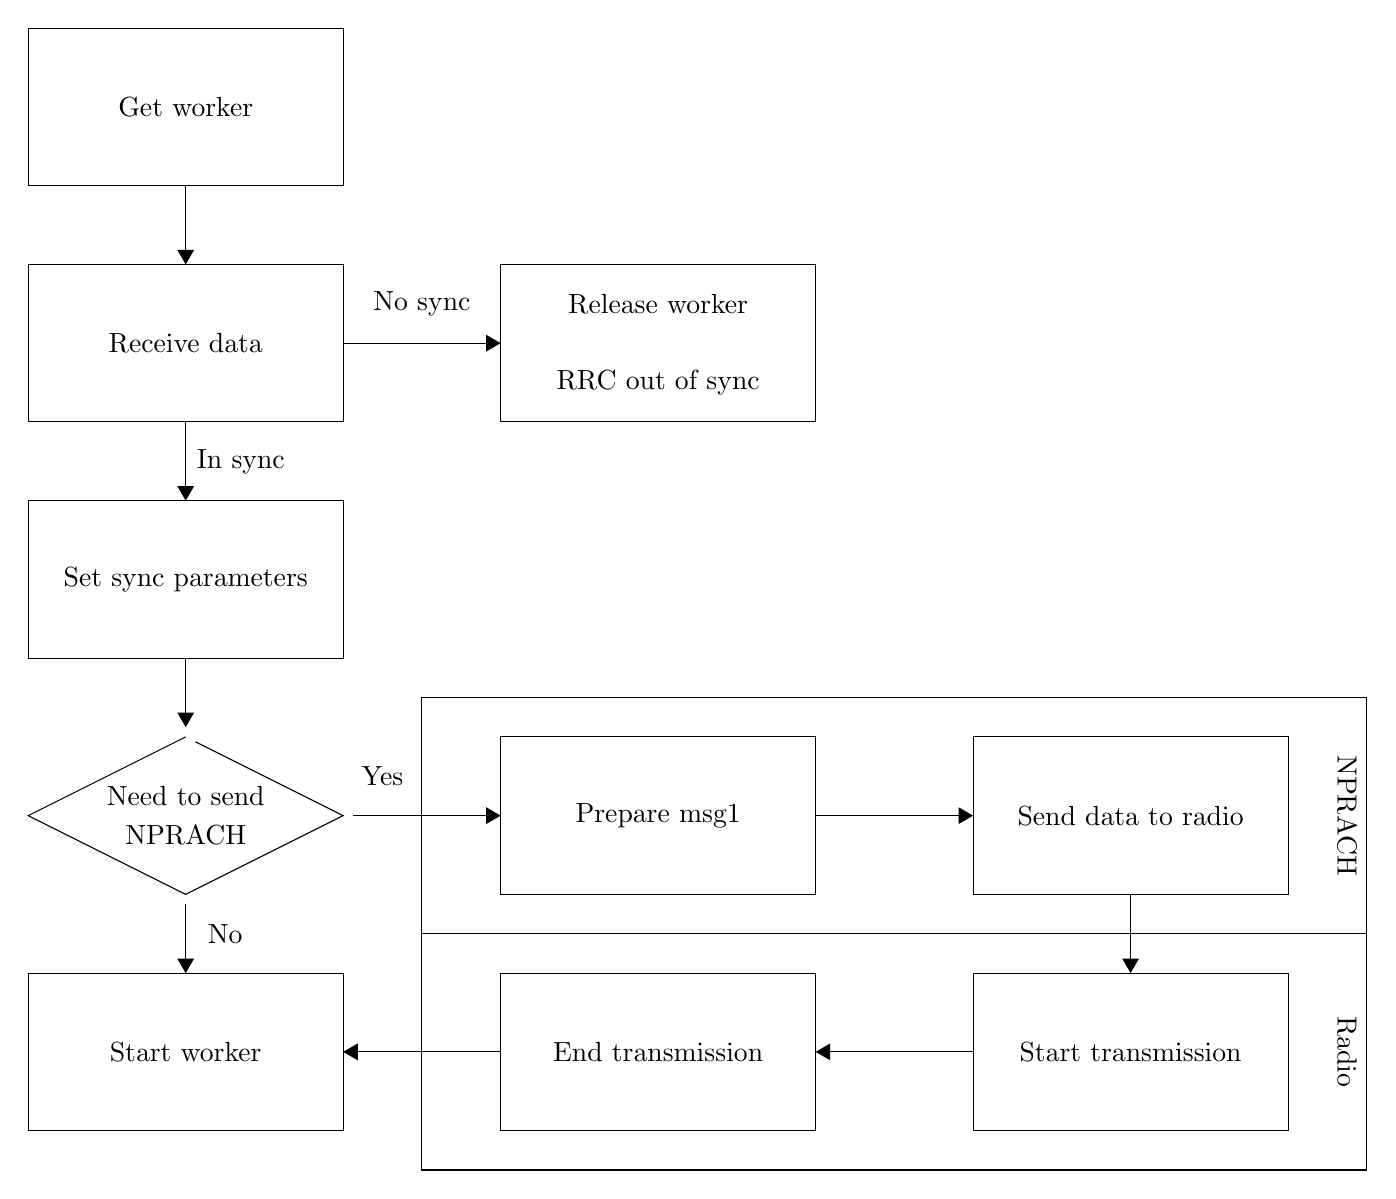
\begin{tikzpicture}

\draw  (-2.5,1.5) rectangle (1.5,-0.5);
\draw  (-2.5,-1.5) rectangle (1.5,-3.5);
\draw  (3.5,-1.5) rectangle (7.5,-3.5);
\draw  (-2.5,-4.5) rectangle (1.5,-6.5);
\draw (-0.5,-7.5) node (v1) {} -- (-2.5,-8.5) -- (-0.5,-9.5) node (v3) {} -- (1.5,-8.5) node (v2) {} -- (v1);
\draw  (-2.5,-10.5) rectangle (1.5,-12.5);
\draw  (3.5,-7.5) rectangle (7.5,-9.5);
\draw  (9.5,-7.5) rectangle (13.5,-9.5);
\draw  (3.5,-10.5) rectangle (7.5,-12.5);
\draw  (9.5,-10.5) rectangle (13.5,-12.5);
\draw  (2.5,-7) rectangle (14.5,-10);
\draw  (2.5,-10) rectangle (14.5,-13);
\draw [-triangle 60](-0.5,-0.5) -- (-0.5,-1.5);
\draw [-triangle 60](1.5,-2.5) -- (3.5,-2.5);
\draw [-triangle 60](-0.5,-3.5) -- (-0.5,-4.5);
\draw [-triangle 60](-0.5,-6.5) -- (v1);
\draw [-triangle 60](v2) -- (3.5,-8.5);
\draw [-triangle 60](7.5,-8.5) -- (9.5,-8.5);
\draw [-triangle 60](11.5,-9.5) -- (11.5,-10.5);
\draw [-triangle 60](9.5,-11.5) -- (7.5,-11.5);
\draw [-triangle 60](3.5,-11.5) -- (1.5,-11.5);
\draw [-triangle 60](v3) -- (-0.5,-10.5);
\node at (-0.5,0.5) {Get worker};
\node at (-0.5,-2.5) {Receive data};
\node at (5.5,-2) {Release worker};
\node at (-0.5,-5.5) {Set sync parameters};
\node at (-0.5,-8.25) {Need to send};
\node at (-0.5,-11.5) {Start worker};
\node at (5.5,-8.5) {Prepare msg1};
\node at (5.5,-11.5) {End transmission};
\node at (11.5,-8.5) {Send data to radio};
\node at (11.5,-11.5) {Start transmission};
\node [rotate=-90] at (14.25,-8.5) {NPRACH};
\node [rotate=-90] at (14.25,-11.5) {Radio};
\node at (2.5,-2) {No sync};
\node at (0.2,-4) {In sync};
\node at (2,-8) {Yes};
\node at (0,-10) {No};
\node at (5.5,-3) {RRC out of sync};
\node at (-0.5,-8.75) {NPRACH};
\end{tikzpicture}